\documentclass[12pt, twoside, openany]{book}

\usepackage{mathptmx} % Contiene una fuente similar a Times New Roman

\usepackage[spanish, es-tabla]{babel} % Permite escritura en castellano
\usepackage[utf8]{inputenc} % Permite utilizar caracteres UTF8

\usepackage{graphicx} % Para la inclusión de gráficos e imágenes
\graphicspath{ {images/} } % Ruta para buscar las imágenes
\usepackage[a4paper,top=30mm,left=30mm,right=25mm,bottom=25mm,headheight=20mm]{geometry} % Configuración de los margenes de la página

% Paquetes para que funcione el formato.
\usepackage{titlesec}
\usepackage{setspace}
\usepackage{ragged2e}
\usepackage{fancyhdr}
\usepackage{lastpage}
\usepackage{stackengine}
\usepackage{array}
\usepackage{hyperref}
\usepackage{enumitem}
\usepackage{float}

\usepackage{hyperref} % Paquete para que las referencias funcionen, y permite introducir links
\usepackage{xcolor} % Paquete para trabajar con colores (fondo de celdas, color del texto...)
\usepackage{pdfpages} % Paquete para incluir páginas de otro PDF directamente
% Se define un color gris desde su código RGB
\definecolor{gris}{RGB}{220,220,220}

\setcounter{secnumdepth}{3} % Para permitir numerar las sub-subsecciones

% Modifica el nombre de los índices al castellano
\addto\captionsspanish{
  \renewcommand{\contentsname}{Índice de contenido}
  \renewcommand{\listfigurename}{Índice de figuras}
  \renewcommand{\listtablename}{Índice de tablas}
}

% Formateo de los nombres de los apartados:
\titleformat{\chapter}[block]
  {\normalfont\Huge\bfseries\singlespacing}{\thechapter.}{1em}{\Huge}
\titlespacing*{\chapter}{0pt}{-62pt}{0pt}

\titleformat{\section}[block]
  {\normalfont\Large\bfseries}{\thesection.}{4pt}{\Large}
\titlespacing*{\section}{0pt}{\baselineskip}{0pt}

\titleformat{\subsection}[block]
  {\normalfont\large\bfseries}{\thesubsection.}{4pt}{\normalsize\large}
\titlespacing*{\subsection}{0pt}{0pt}{0pt}

\titleformat{\subsubsection}[block]
  {\normalfont\normalsize\bfseries}{\thesubsubsection.}{4pt}{\normalsize}
\titlespacing*{\subsubsection}{0pt}{0pt}{0pt}

\def\tablename{Tabla}

%% Variables para portada y cabeceras
%% Cambiar los valores para cada documento!!!
\def\title{Minería de anomalías}
\def\subject{Inteligencia de Negocio}
\def\author{Juan Francisco Mier Montoto}
\def\target{www.mier.info}
\def\authorid{UO283319}
\def\date{diciembre 2023}
\def\org{Escuela Politécnica de Ingeniería de Gijón}
\def\area{Grado en Ingeniería Informática en Tecnologías de la Información}

\def\ORG{\expandafter\MakeUppercase\expandafter{\org}}
\def\AREA{\expandafter\MakeUppercase\expandafter{\area}}
\def\SUBJECT{\expandafter\MakeUppercase\expandafter{\subject}}

\setlength{\headheight}{65pt}

\fancyhf{}
\fancyhead[L]{
\includegraphics[height=16mm]{style/square.png}
  \hspace{1em} \Longstack[l] {
    \textbf{\SUBJECT} \newline
    \textbf{\title}}
  \newline \leftmark{}
}
\fancyhead[R]{\bfseries{Hoja \thepage{}~de~\pageref{LastPage}}}
\fancyfoot[C]{\href{\target}{\author}}
\renewcommand{\headrulewidth}{0pt} % default is 0pt
\renewcommand{\footrulewidth}{0.4pt} % default is 0

\fancypagestyle{plain}{%
  \fancyhf{}
  \fancyhead[L]{
\includegraphics[height=16mm]{style/square.png}
    \hspace{1em} \Longstack[l]{
      \textbf{\SUBJECT} \newline
      \textbf{\title}}}
  \fancyhead[R]{\bfseries{Hoja \thepage{}~de~\pageref{LastPage}}}
  \fancyfoot[C]{\href{\target}{\author}}
  \renewcommand{\headrulewidth}{0pt} % default is 0pt
  \renewcommand{\footrulewidth}{0.4pt} % default is 0pt
}

\pagestyle{fancy}

\restylefloat{table}



\begin{document}

\rmfamily % Fuente tipo Romana

% Portada de la memoria
\begin{titlepage}
    \centering
    \bfseries {
        \null{}
        \vspace{0cm}
        \begin{table}[h]
            \centering
            \begin{tabular}{m{10cm} m{1cm} m{3cm}}
                \vspace{0.2cm}
                
\includegraphics[width=86mm]{style/full.png} &  & \vspace{1.52mm} 
\includegraphics[width=23mm]{style/square.png} \\
            \end{tabular}
        \end{table}

        \vspace{3\baselineskip}

        \Large{\ORG{} \\ \vspace{3\baselineskip}}
        \large {
            \AREA{} \\ \vspace{3\baselineskip}
            \subject{} \\ \vspace{2\baselineskip}

            % TRABAJO FIN DE GRADO/MÁSTER Nº XXXXXXXXX \vspace{\baselineskip} \\
            \title{} \\ \vspace{3\baselineskip}

            \author{} \\
            \authorid{} \\
            % TUTOR/ES: \\
            % D. APELLIDO1 APELLIDO2, Nombre \\
            % D. APELLIDO1 APELLIDO2, Nombre \\  \vspace{\baselineskip}

            \vspace{2\baselineskip}
            FECHA:\@ \date{}
        }
    }
\end{titlepage}


% Índice de contenido
\addcontentsline{toc}{chapter}{Índice de contenido} % Añade la referencia al índice de contenido
\tableofcontents
\newpage

% Índice de figuras
\addcontentsline{toc}{chapter}{Índice de figuras}  % Añade la referencia al índice de contenido
\listoffigures

\justify{} % Texto justificado
\setlength{\parskip}{\baselineskip} % Separación entre párrafos de 1 linea
\onehalfspacing{}

%% El contenido de la memoria, dividido en capítulos:
\chapter{Introducción}
\section{Definiciones}
\subsection{Minería de anomalías}
En esencia, la minería de anomalías (también conocida como \textit{minería de excepciones} o
\textit{detección de valores atípicos}) es una rama de la minería de datos que se enfoca en
la detección de patrones anómalos o inusuales en los datos.

Estas anomalías representan desviaciones significativas de los comportamientos esperados
o de las tendencias habituales en un entorno comercial.
\subsection{Anomalía}
Existen múltiples posibles definiciones de anomalía. Algunas de ellas son:
\begin{itemize}[topsep=0pt]
	\item Una observación que se desvía tanto de las demás como para despertar sospechas de
		que se ha generado por un mecanismo diferente.
	\item Casos o conjuntos de datos que aparecen muy raramente y cuyas características
		difieren significativamente de los demás.
	\item Patrones en los datos que no se ajustan a una noción bien definida de comportamiento
		normal.
\end{itemize}

\section{Objetivos y aplicaciones en el mundo real}
El objetivo principal radica en identificar estos eventos ``atípicos'' que podrían llegar
a indicar problemas o posibles oportunidades, si lo observamos desde el punto de vista de
la \subject.

En el mundo real, la minería de anomalías se puede aplicar (y se aplica) a la hora de
tomar decisiones empresariales, como por ejemplo al detectar fraudes, revelar áreas de
mejora, detectar problemas operativos\ldots

En apartados posteriores se verán ejemplos de aplicaciones y casos de uso de la minería de
excepciones.~(Ver \nameref{chap:cus})

\section{Causas de las anomalías}
Las anomalías pueden ser causadas por una amplia variedad de razones, pero existen algunas
causas comunes que pueden ser identificadas:

\begin{itemize}
	\item \textbf{Datos de clases diferentes:} un objeto puede ser diferente del resto por
		pertencer a una clase diferente. En el ejemplo de los fraudes, los objetos ``outliers''
		dentro de un conjunto de datos pueden ser considerados como inusuales o como potenciales
		fraudes.
	\item \textbf{Variación natural:} cuando los datos se pueden modelar estadísticamente
		mediante una distribución, los objetos que se encuentran en las colas de la distribución
		se pueden llegar a considerar como anomalías.
	\item \textbf{Errores en la medición:} todos los datos que se recogen están sometidos a una
		componente humana y, por lo tanto, a errores. Dichos errores pueden llegar a ser
		considerados anomalías, por lo que hay que lidiar con ellos en la fase de preprocesamiento.
		(Ver \nameref{chap:pre})
\end{itemize}

\section{Historia y evolución}\label{sec:hist}
El concepto de \textit{detección de intrusiones} (IDS) fue introducido por Dorothy Denning en
1987~\cite{denning1987intrusion}. En su trabajo, Denning propuso un sistema de detección de intrusiones
basado en el análisis de los registros de auditoría del sistema. Este sistema se basaba en la idea
de que las actividades de los usuarios legítimos del sistema se pueden modelar y, por lo tanto,
se pueden detectar las actividades que no se ajustan a dicho modelo. Este trabajo fue el punto de
partida de la detección de anomalías.

La detección de intrusiones es un componente crítico de la detección de anomalías y ha ido evolucionando
significativamente con el paso del tiempo. En la actualidad, los sistemas de detección de intrusiones
se basan en técnicas de aprendizaje automático y de minería de datos, reflejando el progreso de la minería
de excepciones.

El término \textit{minería de anomalías} fue introducido por primera vez por \textit{Patcha y Park} en 2007
~\cite{patcha2007overview}.

\chapter{Técnicas y métodos de detección}\label{chap:tecnicas}
Existe una gran variedad de técnicas y métodos de detección de anomalías, si bien cada uno
de ellos tiene sus propias ventajas y desventajas. Es importante tener en cuenta que la
efectividad de cada uno de ellos depende en gran medida del tipo de datos que se esté
tratando, además del propio método en sí.

Por ejemplo, algunos algoritmos de detección están diseñados para detectar anomalías \textit{locales},
mientras que otros están diseñados para detectar anomalías \textit{globales}. Casi todos los algoritmos
requieren que se establezan parámetros de entrada poco intuitivos o incluso desconocidos previo
al propio análisis de los datos, como el número de vecinos más cercanos o umbrales de distancia.

\section{Categorías y etiquetas de clase}
Existen tres grandes categorías de tećnicas de detección de anomalías, dependiendo de la información
sobre los datos de la que se disponga:

\begin{itemize}[topsep=0pt]
	\item \textbf{Detección supervisada:} estas técnicas requieren un conjunto de datos etiquetado
		que contenga tanto datos normales como datos anómalos. El objetivo de estas técnicas es
		crear un \textit{clasificador} que sea capaz de distinguir entre ambos tipos de datos. \\
		Este enfoque no se utiliza frecuentemente, ya que en la práctica es muy difícil obtener
		un conjunto de datos etiquetado por la naturaleza de los datos que se quieren analizar.
	\item \textbf{Detección no supervisada:} cuando no se dispone de datos etiquetados, se puede
		tratar de asociar una \textit{\textbf{puntuación}} a cada objeto en función de la probabilidad que
		se estime de que dicho objeto sea una anomalía. En este caso, no se puede distinguir entre
		diferentes tipos de anomalías, sino que se trata de detectar cualquier tipo de anomalía. \\
		Para que este enfoque funcione, debe existir una diferencia significativa entre los datos
		normales y los considerados \textit{anómalos}.
	\item \textbf{Detección semi-supervisada:} este conjunto de técnicas se puede utilizar cuando se
		cuentan con datos categorizados como \textit{normales} pero NO datos etiquetados como anómalos.
		En este caso, se utiliza un algoritmo para asignar un grado de anormalidad a cada objeto en
		funciónde la información que se tenga de los datos normales. Normalmente, se entrena un
		modelo con los datos normales y se decide si un objeto es anómalo o no si se ajusta al modelo.
\end{itemize}

\section{Enfoques}
Para tratar de resolver el problema de la detección, se han desarrollado una gran variedad de
técnicas y métodos. Los siguientes enfoques son los más comunes:
\begin{itemize}[topsep=0pt]
	\item \textbf{Técnicas basadas en modelos (\textit{estadísticas}):} en este caso, los anomalías serán
		aquellos objetos que no se ajusten bien al modelo que se haya generado previamente. Por ejemplo,
		si se están trabajando en un problema de regresión, las anomalías serán aquellas que tengan un
		gran error de predicción. Dentro de la detección estadística, se distinguen varios tipos de detección:
		(\textbf{probabilística}, \textbf{de outliers} y \textbf{de \textit{novelties}}). Normalmente, se
		trabaja asumiendo que los datos siguen una distribución normal, lo que permite utilizar la media y la
		desviación en problemas univarpiantes o la distancia de \emph{Mahalanobis}~\cite{mahalanobis2018generalized}
		en problemas multivariantes.

		\begin{minipage}{\linewidth}
			\centering
			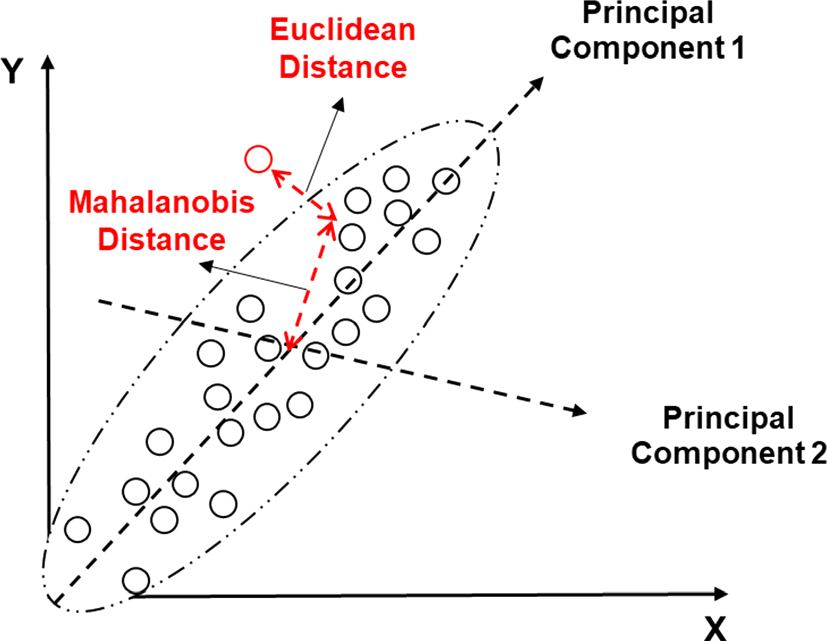
\includegraphics[width=\textwidth]{mahalanobis.png}
			\captionof{figure}{Distancia de Mahalanobis ($T^2$)
				y Euclídea ($Q$)~\cite{lee2020monitoring}}\label{fig:fig2}
		\end{minipage}
	\item \textbf{Técnicas basdadas en proximidad:} estas técnicas explotan una métrica de
		similaridad entre objetos para medir la \textit{distancia} entre ellos. Los objetos que
		se encuentren a una distancia mayor que un umbral establecido se considerarán anomalías.
		En caso de que se pueda representar los datos en un espacio bidimensional, se pueden
		detectar las anomalías a simple vista. La técnica más común es la de los $k$ vecinos más
		cercanos.

		\begin{minipage}{\linewidth}
			\centering
			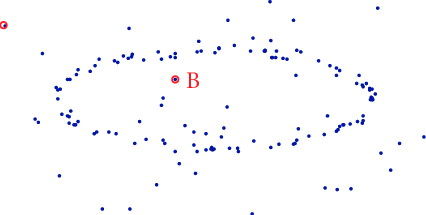
\includegraphics[width=\textwidth]{distance.png}
			\captionof{figure}{Dos tipos distintos de anomalías en la representación de un modelo
				de detección basado en proximidad~\cite{yu2010two}}\label{fig:fig4}
		\end{minipage}
	\item \textbf{Técnicas basadas en densidad:} considerando la densidad como \emph{el número de
		objetos en una región del espacio de datos}, los objetos que se encuentren en regiones
		con una baja densidad se pueden llegar a considerar anómalos. Normalmente se compara la
		densidad de un objeto con la densidad media de los objetos que se encuentran a su alrededor
		(vecinos más cercanos).
	\item \textbf{Técnicas basadas en clusters:} estas técnicas se basan en la idea de que los
		objetos normales pertenecen a un cluster o grupo, mientras que los objetos anómalos no
		pertenecen a ninguno. Por lo tanto, se puede detectar una anomalía si un objeto no pertenece
		a ningún cluster o si pertenece a un cluster con un número muy pequeño de objetos.
		\vspace{1\baselineskip} z

		\begin{minipage}{\linewidth}
			\centering
			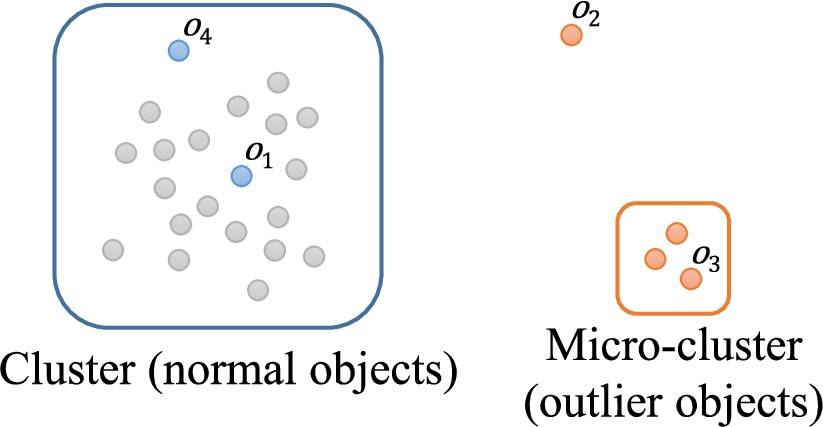
\includegraphics[width=\textwidth]{clusters.png}
			\captionof{figure}{Anomalías en un sistema de detección basado en
				clusters.~\cite{bae2020effective}}\label{fig:fig5}
		\end{minipage}
\end{itemize}

Dentro de los enfoques anteriores, se distinguen una gran variedad de técnicas más:
\begin{itemize}[noitemsep,topsep=0pt]
	\item Redes bayesianas
	\item Redes neuronales (replicantes, autocodificadores, de memoria a corto plazo)
	\item Modelos ocultos de Makarov (\textit{HMM})
	\item Técnicas de ensamblaje (usando \textit{feature bagging})
	\item Basadas en lógica difusa
	\item \textit{SVM} de una clase
	\item \textit{entre otros}
\end{itemize}

Como anteriormente se ha mencionado, el rendimiento de cada una de estas técnicas depende
en gran medida del conjunto de datos y los parámetros escogidos, y no existe una ventaja
clara cuando se comparan entre sí utilizando muchos conjuntos de datos.~\cite{chandola2009anomaly}

\begin{minipage}{\linewidth}
	\centering
	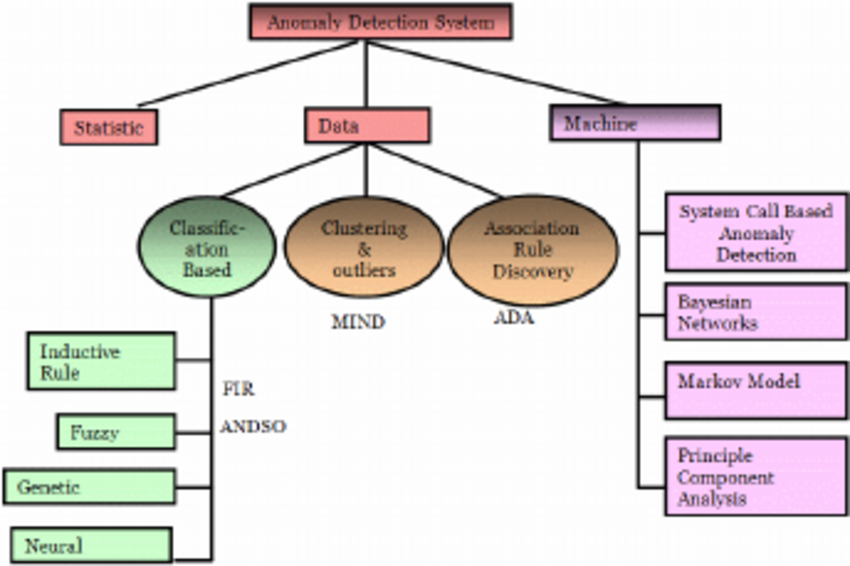
\includegraphics[width=\textwidth]{tecnicas.png}
	\captionof{figure}{Diagrama de técnicas de minería de
		anomalías.~\cite{naz2011multi}}\label{fig:fig8}
\end{minipage}

\chapter{Preprocesamiento de datos}\label{chap:pre}
\section{Técnicas de preprocesamiento}

\section{Selección de características}

\chapter{Casos de uso}
\label{chap:cus}
\section{Casos reales}

\section{Ejemplos de uso}

\chapter{Desafíos y consideraciones éticas}
\section{Problemas comunes}\label{sec:issues}
A la hora de tratar de utilizar y evaluar métodos de detección de anomalías, existen una
serie de problemas comunes que se deben tener en cuenta:

\begin{itemize}[topsep=0pt]
	\item \textbf{Evaluación:} a la hora de evaluar la calidad de un clasificador, las medidas que se tomen
		pueden no ser adecuadas para el problema en cuestión. Por ejemplo, en el caso de los fraudes,
		la tasa de falsos positivos puede ser más importante que la tasa de falsos negativos.
	\item \textbf{Eficiencia y escalabilidad:} debido a la gran cantidad de datos que se manejan y los
		recursos computacionales que se necesitan para crear un clasificador ajustado a estos, la eficiencia
		es un factor a tener en cuenta.
	\item \textbf{Número de atributos:} dependiendo del conjunto de datos con el que se esté tratando, en
		ocasiones puede ser necesario \emph{más de un atributo} para \textbf{definir} una anomalía.
	\item \textbf{Localidad:} a la hora de detectar anomalías, es importante tener en cuenta tanto el
		\emph{conjunto} como el \emph{entorno} en el que se encuentra cada objeto. Como visto en clase,
		una persona puede ser considerada ``anormalmente'' alta para la población \textit{normal},
		pero no dentro del conjunto \textit{jugadores de baloncesto}.
	\item \textbf{Grado de anormalidad:} la propiedad de ser anormal no es binaria, sino que se le puede
		asignar un \emph{grado de anormalidad}, que normalmente define la distancia entre el objeto y el
		conjunto de datos normales. Este concepto es importante y es la base de muchas técnicas de detección
		no supervisadas o semi-supervisadas (Ver \nameref{chap:tecnicas}).
	\item \textbf{Múltiples anomalías simultáneas:} en ocasiones, un objeto puede ser considerado anómalo
		por múltiples razones. En relación con el punto anterior, el hecho de que dos objetos tengan el mismo
		\textit{grado} de anormalidad no implica que sean anómalos por los mismos motivos (\textit{atributos}).
\end{itemize}
\newpage{}
Estos son algunos de los posibles problemas que se pueden encontrar a la hora de desarrollar un sistema de
este tipo, pero existen muchos más:
\begin{itemize}
	\item Preprocesado incorrecto o insuficiente
	\item Conjuntos desbalanceados
	\item Sesgo (Ver \nameref{sec:etica})
	\item Interpretación de los resultados
	\item \ldots
\end{itemize}

\section{Aspectos éticos}\label{sec:etica}
Aunque la detección de anomalías sea una herramienta muy poderosa a la hora de identificar
fraudes, errores o problemas, también plantea desafíos éticos a tener en cuenta.

La primera gran categoría de dichos problemas reside en la obtención del conjunto en sí.
A la hora de recoger datos, es importante tener en cuenta la privacidad y confidencialidad
de las partes interesadas en los mismos, ya que puede contener información sensible. Además
de tener en cuenta la privacidad, es importante considerar la legalidad del tratamiento de
dichos datos. Como se ha visto en otras asignaturas de este curso, la toma de decisiones
automatizada sobre individuos o el tratamiento de datos personales se encuentra regulada
por la \textit{Ley Orgánica de Protección de Datos} (LOPD)~\cite{lopd}.

Otra categoría de problemas éticos reside en la calidad del conjunto. En ocasiones, los
conjuntos de datos pueden contener sesgos, ya sea por la forma en la que se han recogido
los datos o por la propia naturaleza de los mismos. Por ejemplo, en el caso de los fraudes,
es posible que los datos que se tengan sobre fraudes sean de un tipo concreto, por lo que
el clasificador no será capaz de detectar fraudes de otro tipo. Este problema se conoce
como \textit{sesgo de selección}. Otro ejemplo de sesgo es el \textit{sesgo de supervivencia},
que se produce cuando los datos que se tienen son de los objetos que han sobrevivido a un
proceso de selección, pero no de los que no lo han hecho.

Por último, es importante tener en cuenta las posibles consecuencias de la minería de
anomalías. En ocasiones, los resultados de la detección de anomalías pueden tener un
impacto negativo en las personas o entidades involucradas. De otra forma, se pueden
obtener resultados incorrectos o mal interpretados, lo que puede llevar a tomar decisiones
erróneas.

Como conclusión, es importante tener en cuenta que la minería de anomalías es una herramienta
muy potente pero con potenciales consecuencias negativas, en especial contra la privacidad
de individuos y otras partes interesadas. A parte de los problemas éticos, también se deben
tener en cuenta los problemas legales que se pueden derivar de su uso.

\chapter{Herramientas y tecnologías utilizadas}
Para el desarrollo de modelos de predicción de minería de excepciones, existen multitud de
herramientas y tecnologías, algunas de ellas de código abierto, que facilitan el proceso de
desarrollo. Este capítulo tiene como objetivo mencionar algunas de estas herramientas y
tecnologías.

\begin{itemize}
	\item \textbf{ELKI} es un toolkit de minería de datos de código abierto escrito en Java. Está
		diseñado para ser utilizado en investigación y en la industria, y es compatible con la mayoría
		de sistemas operativos. Cuenta además con índices de aceleración especiales.
	\item \textbf{PyOD} es una librería de Python de código abierto desarrollada específicamente
		para la detección de anomalías.~\cite{pyod}
	\item \textbf{scikit-learn} es una librería de Python de código abierto que recoge algoritmos
		de detección de anomalías no supervisados. (Ver \nameref{chap:tecnicas})
	\item \textbf{Wolfram Mathematica} es un software de matemáticas que incluye herramientas de
		minería de datos y de aprendizaje automático de conjuntos de datos de varios
		tipos.~\cite{wolfram}
\end{itemize}

Además de las herramientas mencionadas, las empresas que necesitan modelos y clasificadores más
complejos suelen recurrir a la creación de herramientas propias que se adapten a sus necesidades
y a los servicios y datos que ya tienen. Algunos ejemplos de estas empresas son las vistas en el
capítulo anterior, como Netflix, Uber, Pinterest o LinkedIn.~(Ver \nameref{sect:reales})

\chapter{Conclusiones}


%% Esto incluirá la bibliografía correctamente en nuestro trabajo
\newpage % En una nueva página
\addcontentsline{toc}{chapter}{Bibliografía} % Añade la referencia al índice de contenido

\bibliographystyle{ieeetr} % Define el estilo de la bibliografía
\bibliography{biblio} % Indica el archivo que contiene la colección de citas

\nocite{apuntes}
\nocite{leal2009aplicacion,perez2020uso}
\nocite{enwiki:1188321736,eswiki:155256141}

\end{document}
